\begin{figure}[htb]
    \centering
    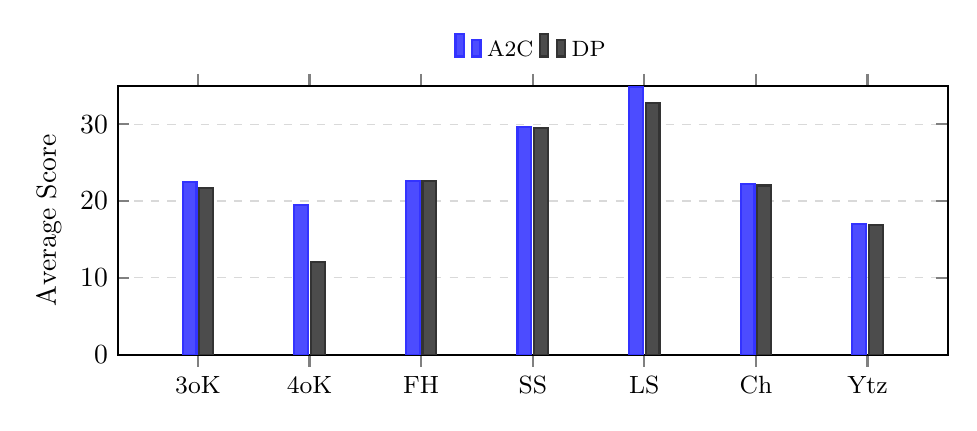
\begin{tikzpicture}
        \begin{axis}[
                ybar=1pt,
                width=\columnwidth,
                height=5cm,
                bar width=5pt,
                symbolic x coords={3oK,4oK,FH,SS,LS,Ch,Ytz},
                xtick=data,
                xticklabel style={font=\small},
                ylabel={Average Score},
                ymin=0,
                ymax=35,
                ymajorgrids=true,
                grid style={dashed,gray!30},
                legend style={
                        at={(0.5,1.05)},
                        anchor=south,
                        legend columns=4,
                        font=\footnotesize,
                        draw=none,
                        fill=none
                    },
                enlarge x limits=0.12,
                axis line style={thick},
                tick style={thick},
            ]

            % A2C
            \addplot[fill=blue!70!white, draw=blue!80!white, thick] coordinates {
                    (3oK,  22.42) (4oK,  19.47) (FH,   22.57) (SS,   29.63)
                    (LS,   34.80) (Ch,   22.22) (Ytz,  17.03)
                };


            % PPO
            %\addplot[fill=red!60!white, draw=red!80!white, thick] coordinates {
            %        (3oK,  5) (4oK,  5) (FH,   5) (SS,   5)
            %        (LS,   5) (Ch,   5) (Ytz,  5)
            %    };

            % REINFORCE
            %\addplot[fill=green!60!white, draw=green!80!white, thick] coordinates {
            %        (3oK,  5) (4oK,  5) (FH,   5) (SS,   5)
            %        (LS,   5) (Ch,   5) (Ytz,  5)
            %    };

            % DP
            \addplot[fill=black!70, draw=black!80, thick] coordinates {
                    (3oK,  21.66) (4oK,  12.10) (FH,   22.59) (SS,   29.46)
                    (LS,   32.71) (Ch,   22.01) (Ytz,  16.87)
                };

            \legend{A2C,DP}

        \end{axis}
    \end{tikzpicture}
    \caption{Lower section scores (placeholder data)}
    \label{fig:category-lower}
\end{figure}
